% !TeX root = er.tex

\chapter{Robôs e Suas Aplicações}\label{ch.basic}

Embora todos pareçam saber o que é um robô, é difícil dar uma definição precisa. Em tradução livre, a definição dada pelo \emph{Oxford English Dictionary} é: ``Uma máquina capaz de realizar automaticamente uma série complexa de ações, especialmente uma programável por computador''. Esta definição inclui alguns elementos interessantes:
\begin{itemize}
\item ``Atualização automática das ações''. Este é um elemento chave na robótica, mas também em muitas outras máquinas mais simples chamadas autômatos. A diferença entre um robô e um simples autômato como uma máquina de lavar louça está na definição do que é uma "série complexa de ações". A lavagem de roupas é ou não composta de uma série complexa de ações? Pilotar um avião em um piloto automático é uma ação complexa? Fazer pão é uma ação complexa? Para todas estas tarefas existem máquinas que estão na fronteira entre autômatos e robôs.
\item O item "Programável por computador" é outro elemento chave de um robô, pois alguns autômatos são programados mecanicamente e não são muito flexíveis. Por outro lado, os computadores são encontrados em todos os lugares, portanto é difícil utilizar este critério para distinguir um robô de outra máquina.
\end{itemize}
Um elemento crucial dos robôs que não é mencionado explicitamente na definição é o uso de sensores. A maioria dos autômatos não tem sensores e não podem adaptar suas ações ao seu ambiente. Os sensores são o que permite que um robô execute tarefas complexas. 

Em Sects.~\ref{s.classification}--\ref{s.educational} deste capítulo introdutório fazemos um pequeno levantamento dos diferentes tipos de robôs. A seção ~\ref{s.generic} descreve o robô genérico que usamos e a seção Sect.~\ref{s.alg-formalism} apresenta o pseudocódigo usado para formalizar os algoritmos. A seção~\ref{s.overview} dá uma visão detalhada do conteúdo do livro.

\section{Classificação de Robôs}\label{s.classification}

Os robôs podem ser classificados de acordo com o ambiente em que operam (Fig.~\ref{fig.classification1}). A distinção mais comum é entre os robôs \emph{fixos} e \emph{móveis}. Estes dois tipos de robôs têm ambientes de trabalho muito diferentes e, portanto, requerem capacidades muito diferentes. Os robôs fixos são, em sua maioria, manipuladores robóticos industriais que trabalham em ambientes bem definidos e adaptados para robôs. Esses robôs industriais executam tarefas repetitivas específicas, como soldagem ou pintura de peças em fábricas de automóveis. Com o aperfeiçoamento dos sensores e dispositivos para interação homem-robô, os manipuladores robóticos são cada vez mais utilizados em ambientes menos controlados, como cirurgia de alta precisão.

\begin{figure}
\begin{center}
% Classification of robots according to environment
\begin{tikzpicture}[node distance = 4mm and 1cm]
\node (robot) { \textsf{robô} };
\node (fixed) [below right=of robot] { \textsf{fixo} };
\node (mobile) [above right=of robot] { \textsf{móvel} };
\node (water) [above right=of mobile] { \textsf{aquático} };
\node (land) [right=of mobile] { \textsf{terrestre} };
\node[xshift=-10pt] (air) [below right=of mobile] { \textsf{aéreo} };
\node (wheeled) [above right=of land] { \textsf{a rodas} };
\node[xshift=10pt] (legged) [below right=of land] { \textsf{a patas} };
\draw (robot) -- (fixed);
\draw (robot) -- (mobile);
\draw (mobile) -- (water);
\draw (mobile) -- (land);
\draw (mobile) -- (air);
\draw (land) -- (wheeled);
\draw (land) -- (legged);
\end{tikzpicture}
\end{center}
\caption{Classificação de robôs por ambiente e mecanismo de interação}\label{fig.classification1}
\end{figure}

Em contraste, espera-se que robôs móveis se movimentem e executem tarefas em ambientes grandes, mal definidos e incertos, que não são projetados especificamente para robôs. Eles precisam lidar com situações que não são precisamente conhecidas com antecedência e que mudam com o tempo. Tais ambientes podem incluir entidades imprevisíveis como seres humanos e animais. Exemplos de robôs móveis são os aspiradores de pó robotizados e os veículos autônomos (carros que se auto dirigem). 

Não há uma linha divisória clara entre as tarefas executadas por robôs fixos e móveis - os humanos podem interagir com robôs industriais e os robôs móveis podem ser restringidos a se moverem em pistas - mas é conveniente considerar as duas classes como fundamentalmente diferentes. Em particular, os robôs fixos estão presos a um suporte estável no chão, de modo que podem calcular sua posição com base em seu estado interno, enquanto os robôs móveis precisam confiar em sua percepção do ambiente a fim de calcular sua localização.

Existem três ambientes principais para robôs móveis que requerem princípios de projeto significativamente diferentes porque diferem no mecanismo de movimento: aquático (exploração submarina), terrestre (carros) e aéreo (\emph{drones}). Novamente, a classificação não é rigorosa; por exemplo, existem robôs anfíbios que se movimentam tanto na água quanto no solo. Os robôs para estes três ambientes podem ser ainda mais divididos em subclasses: robôs terrestres podem ter pernas ou rodas ou esteiras, e robôs aéreos podem ser balões mais leves que ar ou aviões mais pesados que o ar, que por sua vez são divididos em asa fixa e asa rotativa (helicópteros).

\begin{figure}
\begin{center}
% Classification of robots according to task
\begin{tikzpicture}[node distance = 6mm and 1cm]
\node[text width=8mm,align=left] (robot) { \textsf{robô} };
\node[text width=12mm,align=left] (industrial) [above right=of robot] { \textsf{industrial} };
\node[text width=12mm,align=left] (service) [below right=of robot] {\textsf{serviço}};
\node[text width=20mm,align=left] (logistics) [above right=of industrial] { \textsf{logística} };
\node[text width=20mm,align=left] (manufacturing) [below=of logistics] { \textsf{fabricação} };
\node[text width=20mm,align=left] (medical) [below=of manufacturing] { \textsf{médico} };
\node[text width=20mm,align=left] (home) [below=of medical] { \textsf{doméstico} };
\node[text width=20mm,align=left] (education) [below=of home] { \textsf{educacional} };
\node[text width=20mm,align=left] (military) [below=of education] {  \textsf{defesa}};
%
\draw (robot.north east) -- (industrial.south west);
\draw (robot.south east) -- (service.north west);
\draw (industrial.north east) -- (logistics.south west);
\draw (industrial.east) -- (manufacturing.west);
\draw (service.north east) -- (medical.south west);
\draw (service.east) -- (home.west);
\draw (service.south east) -- (education.north west);
\draw (service.south east |- 0,-15mm) -- (military.north west);
\end{tikzpicture}
\end{center}
\caption{Classificação de robôs por campo de aplicação}\label{fig.classification2}
\end{figure}

Robôs podem ser classificados pelo campo de aplicação pretendido e pelas tarefas que executam (Fig.~\ref{fig.classification2}). Mencionamos os robôs industriais que trabalham em ambientes bem definidos nas tarefas de produção. Os primeiros robôs foram robôs industriais porque o ambiente bem definido simplificou seu projeto. Robôs de serviço, por outro lado, auxiliam os humanos em suas tarefas. Estes incluem robôs que realizam tarefas domésticas (como aspiradores de pó robóticos), transporte (como veículos autônomos) e aplicações de defesa (como \emph{drones} de reconhecimento). A medicina também tem visto o uso crescente de robôs em cirurgia, reabilitação e treinamento. Estas são aplicações recentes que requerem sensores melhores e uma interação mais próxima com o usuário.

\section{Robôs Industriais}

Os primeiros robôs foram robôs industriais que substituíram trabalhadores humanos executando tarefas simples e repetitivas. As linhas de montagem de uma fábrica podem operar sem a presença de humanos em um ambiente bem definido onde o robô tem de executar tarefas em uma ordem específica, atuando sobre objetos precisamente colocados no seu entorno (Fig.~\ref{fig.assemblyline}). 

\begin{figure}
\begin{center}
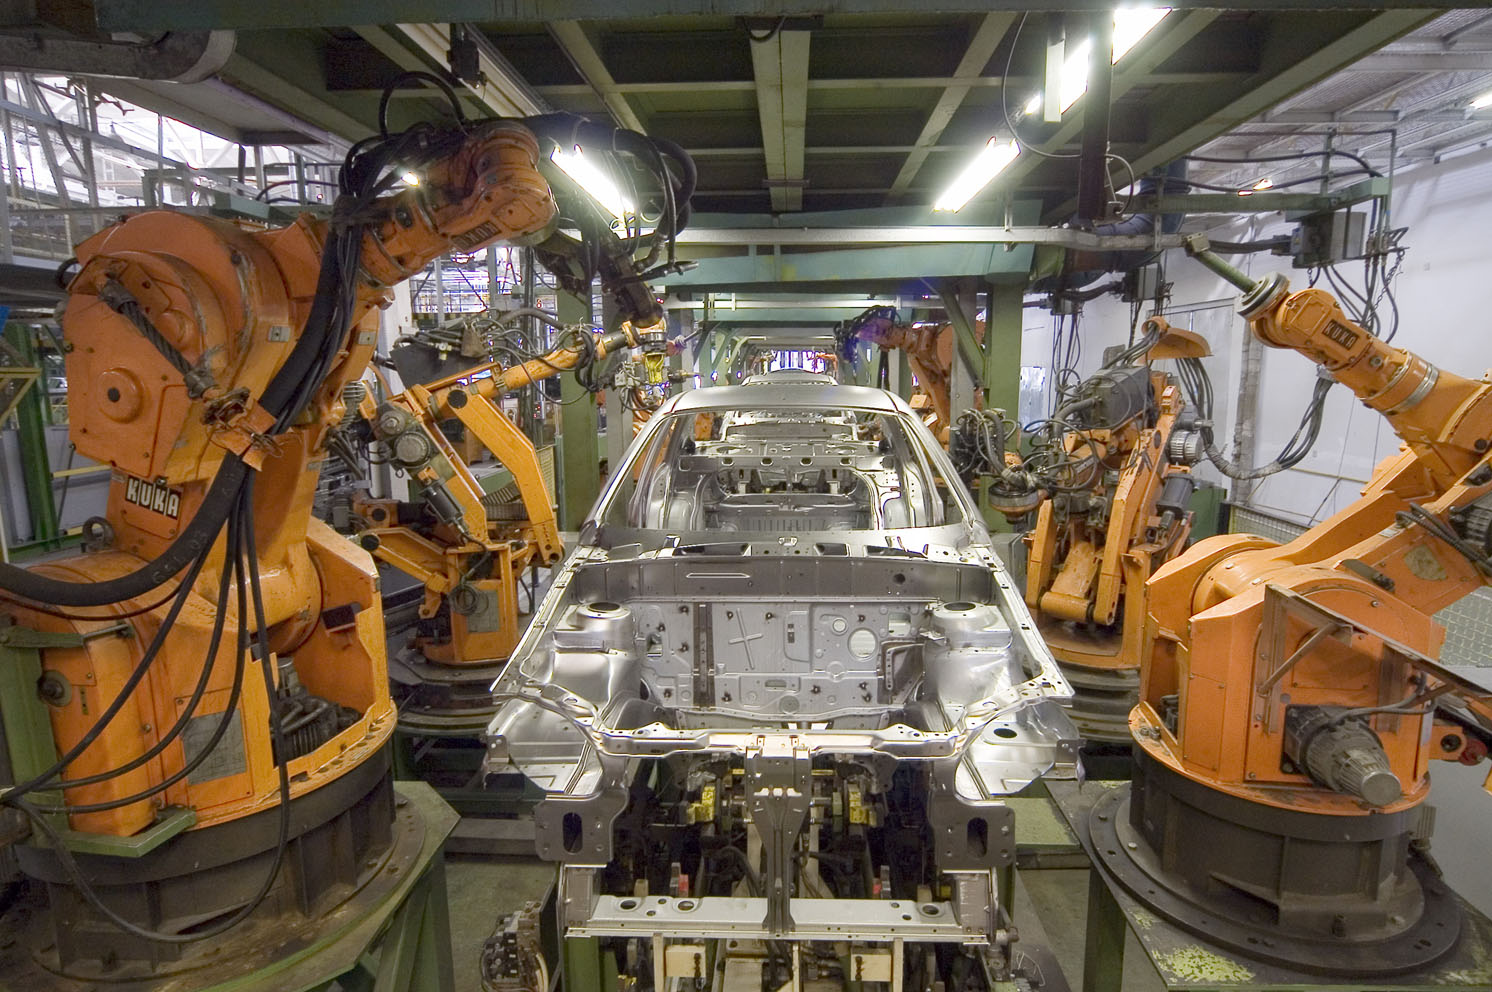
\includegraphics[width=\textwidth]{KUKA_Industrial_Robots_IR_wikimedia.jpg}
\end{center}
\caption{Robôs em uma linha de montagem em uma fábrica de automóveis. Fonte: https://commons.wikimedia.org/wiki/File:AKUKA\_Industrial\_Robots\_IR.jpg por Mixabest (Own work). CC BY-SA 3.0 (http://creativecommons.org/licenses/by-sa/3.0) ou GFDL (http://www.gnu.org/copyleft/fdl.html), via Wikimedia Commons.}\label{fig.assemblyline}
\end{figure}

Poder-se-ia argumentar que estes são realmente autômatos e não robôs. No entanto, os autômatos de hoje muitas vezes dependem de sensores na medida em que podem ser considerados como robôs. No entanto, seu projeto é simplificado porque eles trabalham em um ambiente personalizado ao qual os humanos não têm permissão de acesso enquanto o robô está trabalhando.

Entretanto, os robôs de hoje precisam de mais flexibilidade, por exemplo, a capacidade de manipular objetos em diferentes orientações ou de reconhecer diferentes objetos que precisam ser embalados na ordem correta. O robô pode ser usado para transportar mercadorias de e para  armazéns. Isto traz autonomia adicional, mas a característica básica permanece: o ambiente é mais ou menos limitado e pode ser adaptado ao robô.

Uma flexibilidade adicional é necessária quando os robôs industriais interagem com humanos e isto introduz fortes exigências de segurança, tanto para os braços robóticos quanto para os robôs móveis. Em particular, a velocidade do robô deve ser reduzida e o projeto mecânico deve garantir que as peças móveis não sejam um perigo para o usuário. A vantagem dos humanos trabalhando com robôs é que cada um pode realizar o que faz de melhor: os robôs realizam tarefas repetitivas ou perigosas, enquanto os humanos realizam etapas mais complexas e definem as tarefas gerais do robô, já que são rápidos em reconhecer erros e oportunidades de otimização.

\section{Robôs Móveis Autônomos}

Muitos robôs móveis são controlados remotamente, executando tarefas como inspeção de tubulações, fotografia aérea e eliminação de bombas, mas dependem de um operador que controla o dispositivo. Estes robôs não são autônomos; eles usam seus sensores para dar ao operador acesso remoto a lugares perigosos, distantes ou inacessíveis. Alguns deles podem ser semi-autônomos, executando subtarefas automaticamente. O piloto automático de um drone estabiliza o voo enquanto o humano escolhe a rota de voo. Um robô em um cano pode controlar seu movimento dentro do cano, enquanto o humano procura por defeitos que precisam ser reparados. Os \emph{robôs móveis totalmente autônomos} não dependem de um operador, mas tomam decisões por conta própria e executam tarefas como transportar material enquanto navegam em terrenos incertos (paredes e portas dentro de edifícios, interseções nas ruas) e em um ambiente em constante mudança (pessoas andando, carros movendo-se nas ruas).

Os primeiros robôs móveis foram projetados para ambientes simples, por exemplo, robôs que limpavam piscinas ou cortadores de grama robóticos. Atualmente, os aspiradores de pó robóticos estão amplamente disponíveis porque se provou ser possível construir robôs a preços razoáveis que possam navegar em um ambiente interno repleto de obstáculos.

Muitos robôs móveis autônomos são projetados para apoiar os profissionais que trabalham em ambientes estruturados, como armazéns. Um exemplo interessante é um robô para os campos de capina (Fig.~\ref{fig.agri_robot}). Este ambiente é parcialmente estruturado, mas sensoreamento avançado é necessário para realizar as tarefas de identificação e remoção de ervas daninhas. Mesmo em fábricas muito estruturadas, os robôs compartilham o ambiente com os humanos e, portanto, sua detecção deve ser extremamente confiável.

\begin{figure}
\begin{center}
\includegraphics[width=0.8\textwidth]{ecorobotix.jpg}
\end{center}
\caption{Robô móvel autônomo capinando um campo (cortesia de Ecorobotix)}\label{fig.agri_robot}
\end{figure}

Talvez o tipo de robô móvel autônomo mais publicitado hoje em dia seja o veículo autônomo. Estes são extremamente difíceis de se desenvolver devido ao ambiente altamente complexo e incerto do tráfego motorizado e aos rigorosos requisitos de segurança.

Um ambiente ainda mais difícil e perigoso é o espaço. Os \emph{rovers} Sojourner e Curiosity são robôs móveis semi-autônomos enviados a Marte. O Sojourner esteve ativo por três meses em 1997. O Curiosity está ativo desde seu pouso em Marte em 2012! Enquanto um motorista humano na Terra controla as missões (as rotas para navegação e as experiências científicas a serem conduzidas), esses \emph{rovers} têm a capacidade de evitar riscos de forma autônoma.

Grande parte da pesquisa e desenvolvimento em robótica atualmente está focada em tornar os robôs mais autônomos, melhorando os sensores e permitindo um controle mais inteligente do robô. Melhores sensores podem perceber os detalhes de situações mais complexas mas, para lidar com tais situações, o controle do comportamento do robô deve ser muito flexível e adaptável. A visão computacional, em particular, é um campo de pesquisa muito ativo porque câmeras são baratas e a informação que elas podem adquirir é muito rica. Estão sendo feitos esforços para tornar os sistemas mais flexíveis, para que eles possam aprender com um humano ou adaptar-se a novas situações. Outro campo ativo de pesquisa aborda a interação entre humanos e robôs. Isto envolve tanto a detecção quanto a inteligência, mas também deve levar em conta a psicologia e a sociologia das interações.

\section{Robôs Humanóides}

A ficção científica e os meios de comunicação de massa gostam de representar os robôs de forma humanóide. Todos estamos familiarizados com o R2-D2 e o 3-CPO, os personagens robóticos dos filmes \emph{Star Wars}, mas o conceito tem uma longa história. No século XVIII, um grupo de relojoeiros suíços - Pierre e Henri-Louis Jaquet-Droz e Jean-Fr\'{e}d\'{e}ric Leschot - construíram autômatos humanóides para demonstrar suas habilidades mecânicas e anunciar seus relógios. Muitas empresas hoje constroem robôs humanóides por razões similares.

Robôs humanóides são uma forma de robô móvel autônomo com um projeto mecânico extremamente complexo para mover os braços e para a locomoção por pernas. Os robôs humanóides são usados para pesquisas sobre a mecânica do caminhar e a interação homem-máquina. Robôs humanóides foram propostos para realizar serviços e manutenção em uma casa ou em uma estação espacial. Eles estão sendo considerados para prestar cuidados a idosos que possam se sentir ansiosos na presença de uma máquina que não pareça humana. Por outro lado, robôs que se parecem muito aos humanos podem gerar repulsão, um fenômeno chamado de \emph{uncanny valley}.

Os robôs humanóides podem ser muito difíceis de projetar e controlar. Eles são caros para construir com múltiplas articulações que podem se mover de muitas maneiras diferentes. Robôs que utilizam rodas ou esteiras são preferidos para a maioria das aplicações porque são mais simples, baratos e robustos.

\section{Robôs Educacionais}\label{s.educational}

Os avanços na eletrônica e na mecânica tornaram possível a construção de robôs relativamente baratos. Os robôs educacionais são amplamente utilizados nas escolas, tanto em salas de aula quanto em atividades extracurriculares. O grande número de robôs educacionais torna impossível dar uma visão geral completa. Aqui damos poucos exemplos que são representativos dos robôs comumente usados na educação.

\smallskip

\noindent\textbf{Robôs Móveis Pré-montados}

Muitos robôs educacionais são projetados como robôs móveis pré-montados. A Fig.~\ref{fig.thymio} mostra o robô Thymio da Mobsya e a Fig.~\ref{fig.dash} mostra o robô Dash da Wonder Workshop. Estes robôs são relativamente baratos, robustos e que contêm um grande número de sensores e componentes de saída, tais como luzes. Uma vantagem importante destes robôs é que se pode implementar algoritmos robóticos de imediato, sem investir horas no projeto mecânico e na construção. Entretanto, os robôs pré-montados não podem ser modificados, embora muitos suportem extensões de construção utilizando, por exemplo, componentes \lego{}.

\begin{figure}
\begin{minipage}{.45\textwidth}
\begin{center}
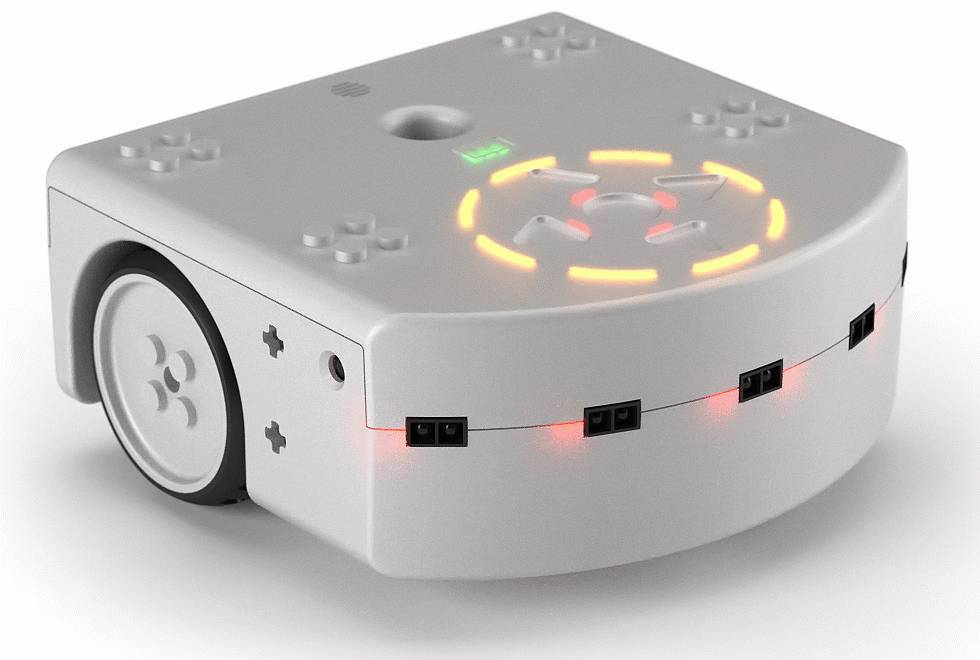
\includegraphics[width=.45\textwidth]{thymio}
\caption{Robô Thymio. Fonte: \protect\url{https://www.thymio.org/en:mediakit} com autorização  de \'{E}cole Polytechnique F\'{e}d\'{e}rale de Lausanne e \'{E}cole Cantonale d'Art de Lausanne.}\label{fig.thymio}
\end{center}
\end{minipage}
\hspace{\fill}
\begin{minipage}{.45\textwidth}
\begin{center}
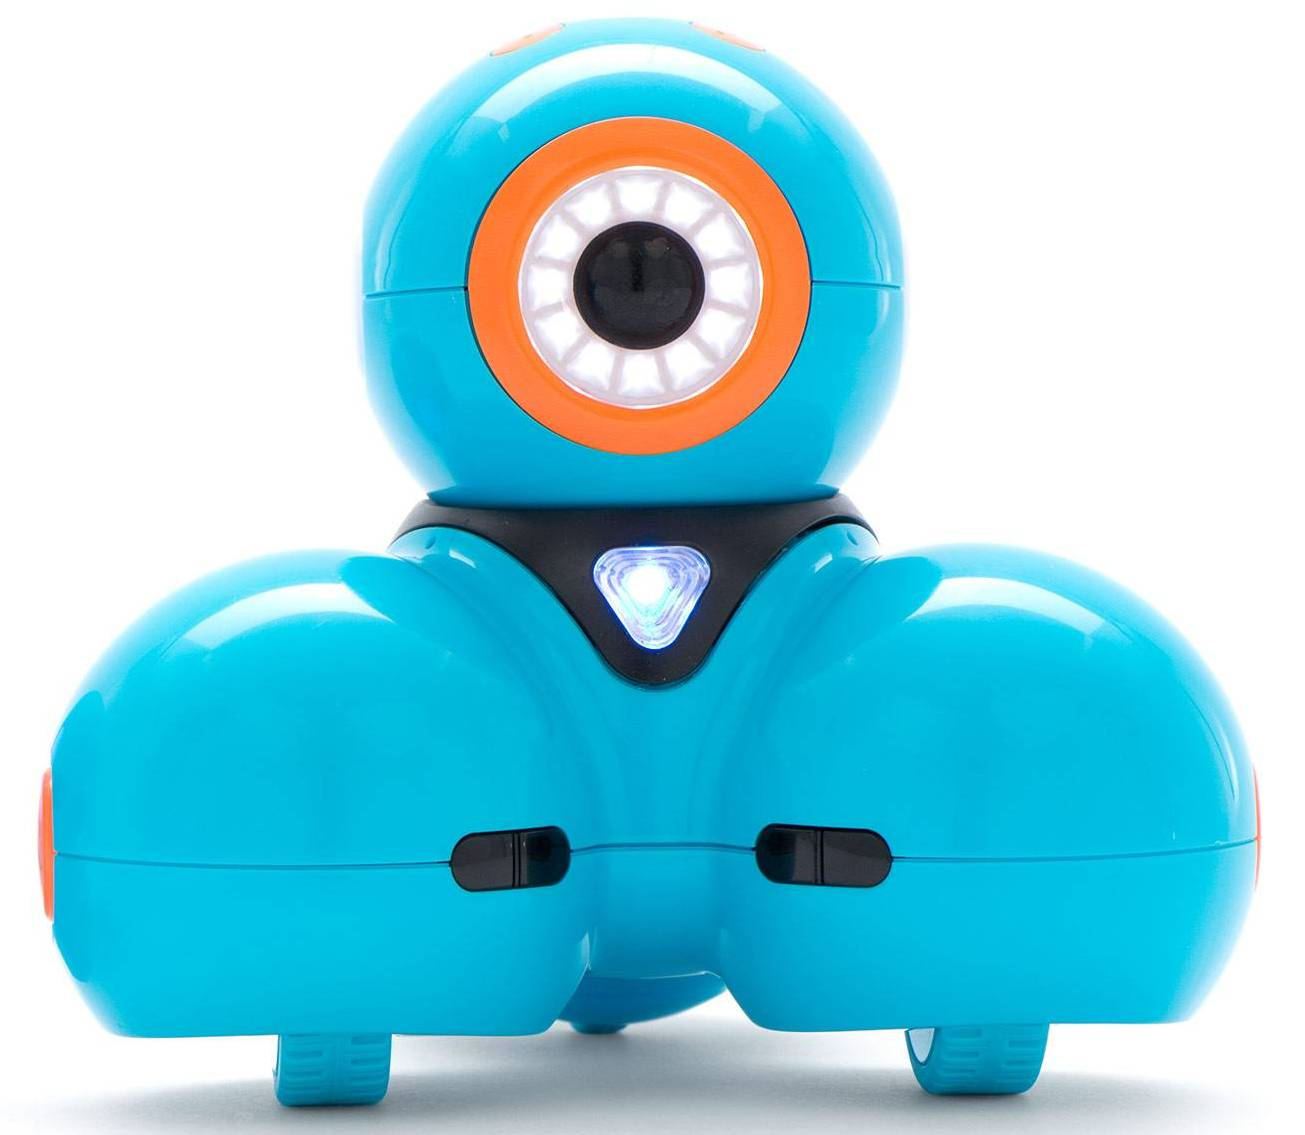
\includegraphics[width=.45\textwidth]{dash}
\caption{Robot Dash. Fonte: \protect\url{https://www.makewonder.com/mediakit} com autorização de Wonder Workshop.}\label{fig.dash}
\end{center}
\end{minipage}
\end{figure}

%
%
%\begin{figure}
%\subfigures
%\begin{minipage}{\textwidth}
%\leftfigure{
%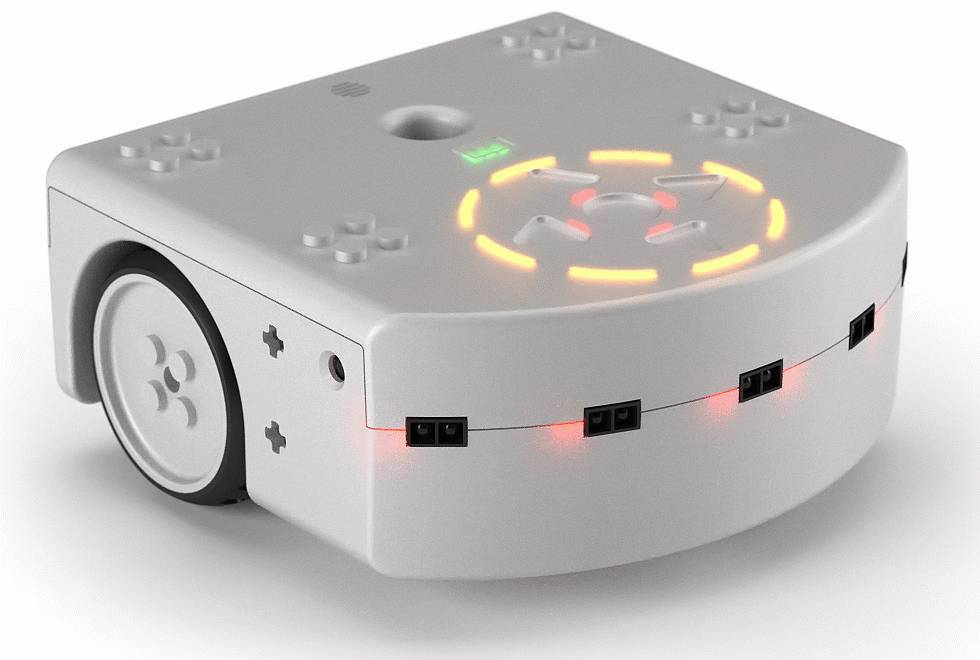
\includegraphics[width=.45\textwidth]{thymio}
%}
%\hspace{\fill}
%\rightfigure{
%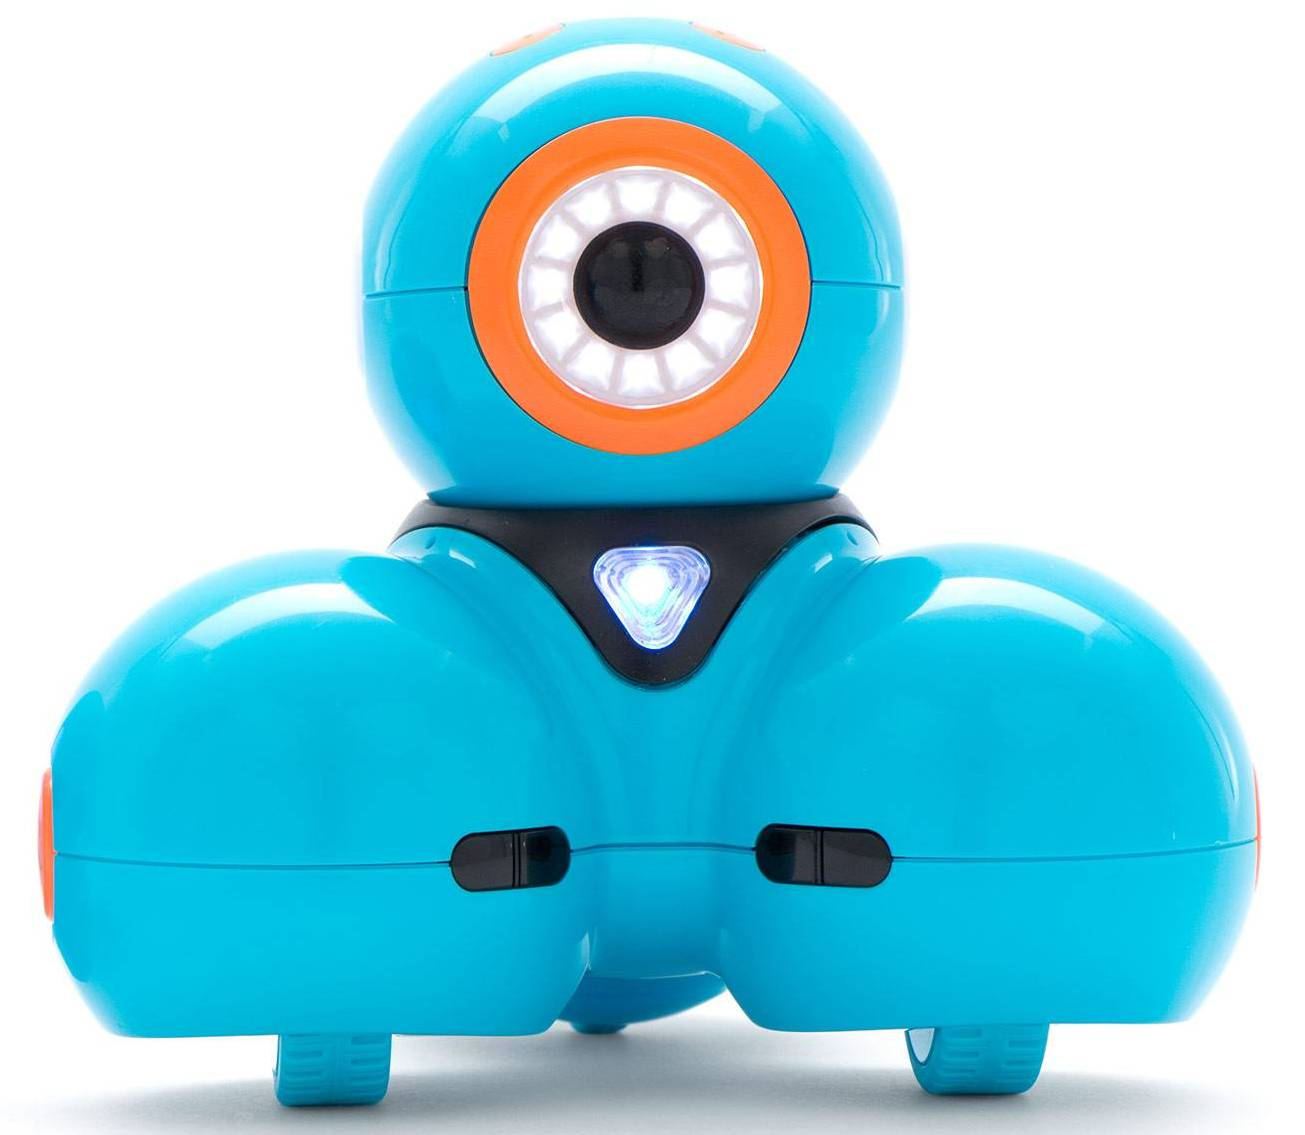
\includegraphics[width=.45\textwidth]{dash}
%}
%\leftcaption{Thymio robot. Source: https://www.thymio.org/en:mediakit by permission of \'{E}cole Polytechnique F\'{e}d\'{e}rale de Lausanne and \'{E}cole Cantonale d'Art de Lausanne.}\label{fig.thymio}
%\rightcaption{Dash robot. Source: https://www.makewonder.com/mediakit by permission of Wonder Workshop.}\label{fig.dash}
%\end{minipage}
%\end{figure}
%
\smallskip

\noindent\textbf{Kits de Robótica}

Os kits robóticos Mindstorms (Fig.~\ref{fig.lego}) foram introduzidos pela \lego{} em 1998.\footnote{A figura mostra a versão chamada \emph{EV3}, introduzida em 2014.} Um kit consiste em blocos e outros componentes de construção padrão, juntamente com motores e sensores, e um bloco programável que contém o computador que controla os componentes do robô. A vantagem dos kits robóticos é que eles são flexíveis: pode-se projetar e construir um robô para realizar uma tarefa específica, limitada apenas pela sua imaginação. Um kit de robótica também pode ser usado para ensinar aos estudantes sobre projeto mecânico. As desvantagens dos kits de robótica são que eles são mais caros do que simples robôs pré-montados e que a exploração de algoritmos de robótica depende da capacidade de se implementar com sucesso um projeto mecânico robusto.

Uma tendência recente é a de substituir coleções fixas de blocos por peças construídas por impressoras 3D. Um exemplo é o braço robótico Poppy Ergo Jr. (Fig.~\ref{fig.poppy}). O uso de peças impressas em 3D permite maior flexibilidade na criação da estrutura mecânica e maior robustez, mas requer acesso a uma impressora 3D. 

\begin{figure}
\begin{minipage}{.45\textwidth}
\begin{center}
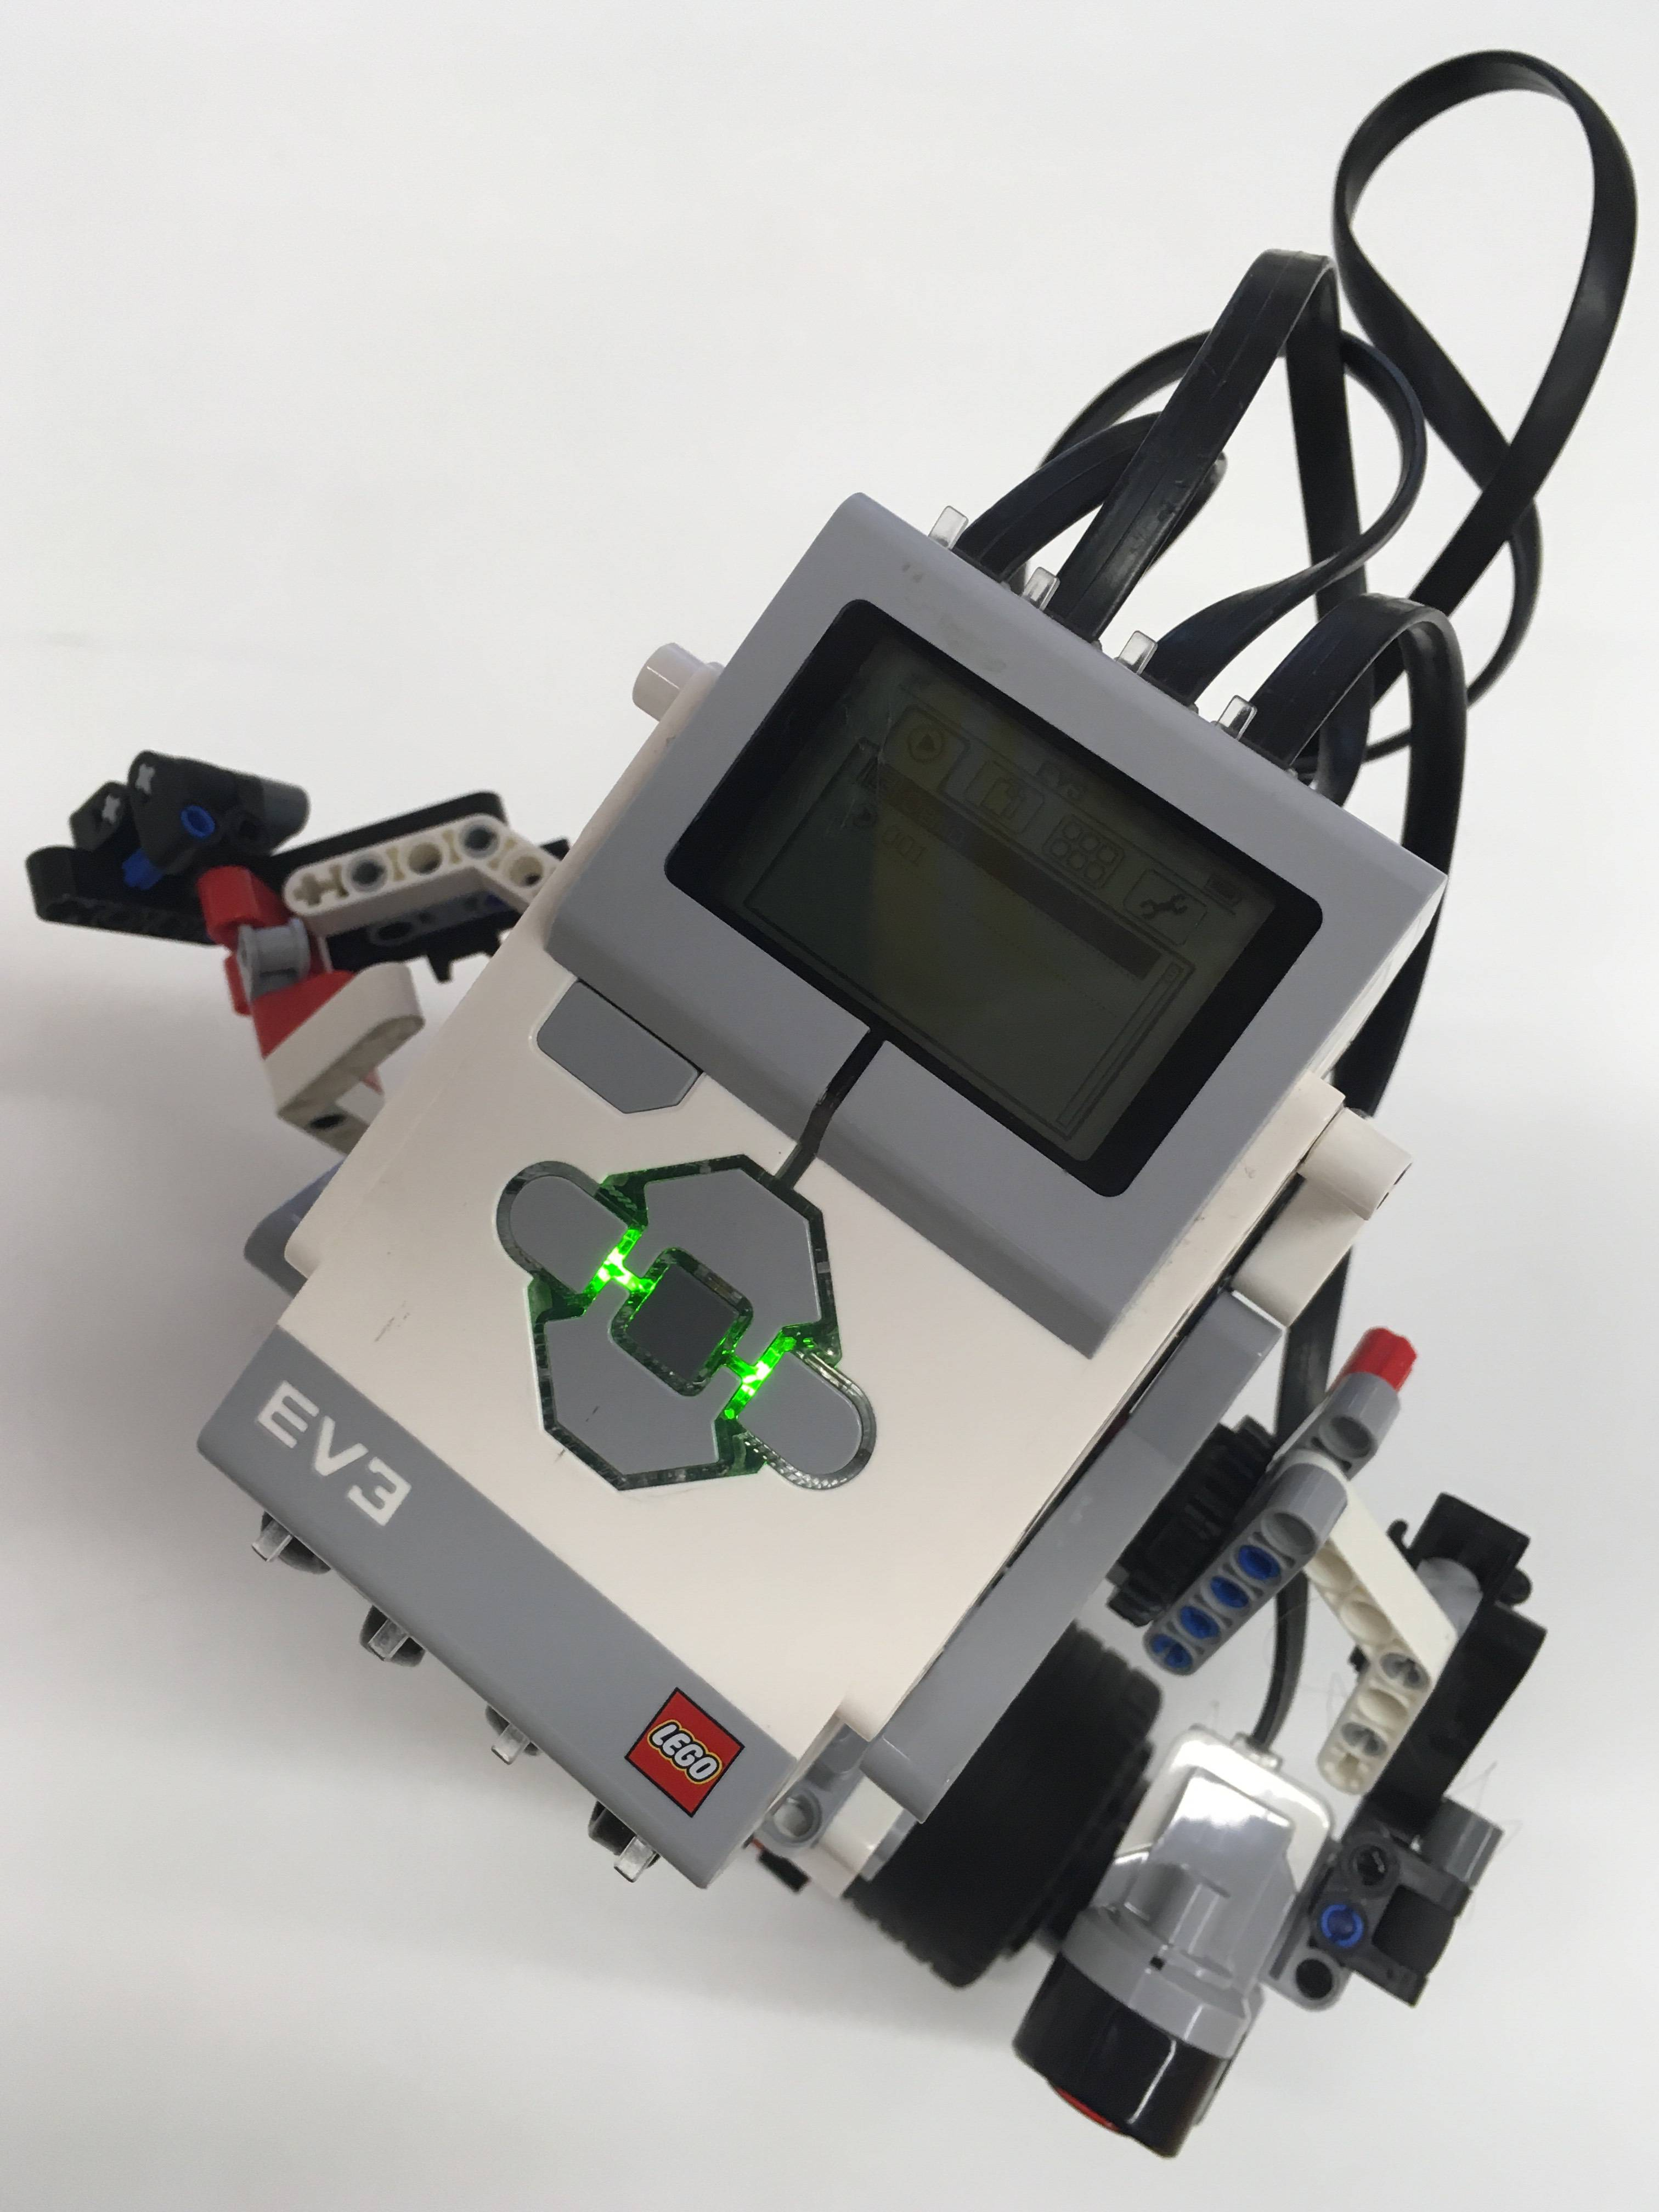
\includegraphics[width=.4\textwidth]{lego}
\end{center}
\caption{\lego{} Mindstorms EV3 (Cortesia de Adi Shmorak, Intelitek)}
\label{fig.lego}
\end{minipage}
\hspace{\fill}
\begin{minipage}{.45\textwidth}
\begin{center}
\includegraphics[width=.55\textwidth]{ErgoJr.jpg}
\end{center}
\caption{Braços robóticos Poppy Ergo Jr (Cortesia de Poppy Project)}
\label{fig.poppy}
\end{minipage}
\end{figure}


%\begin{figure}
%\subfigures
%\begin{minipage}{\textwidth}
%\leftfigure{
%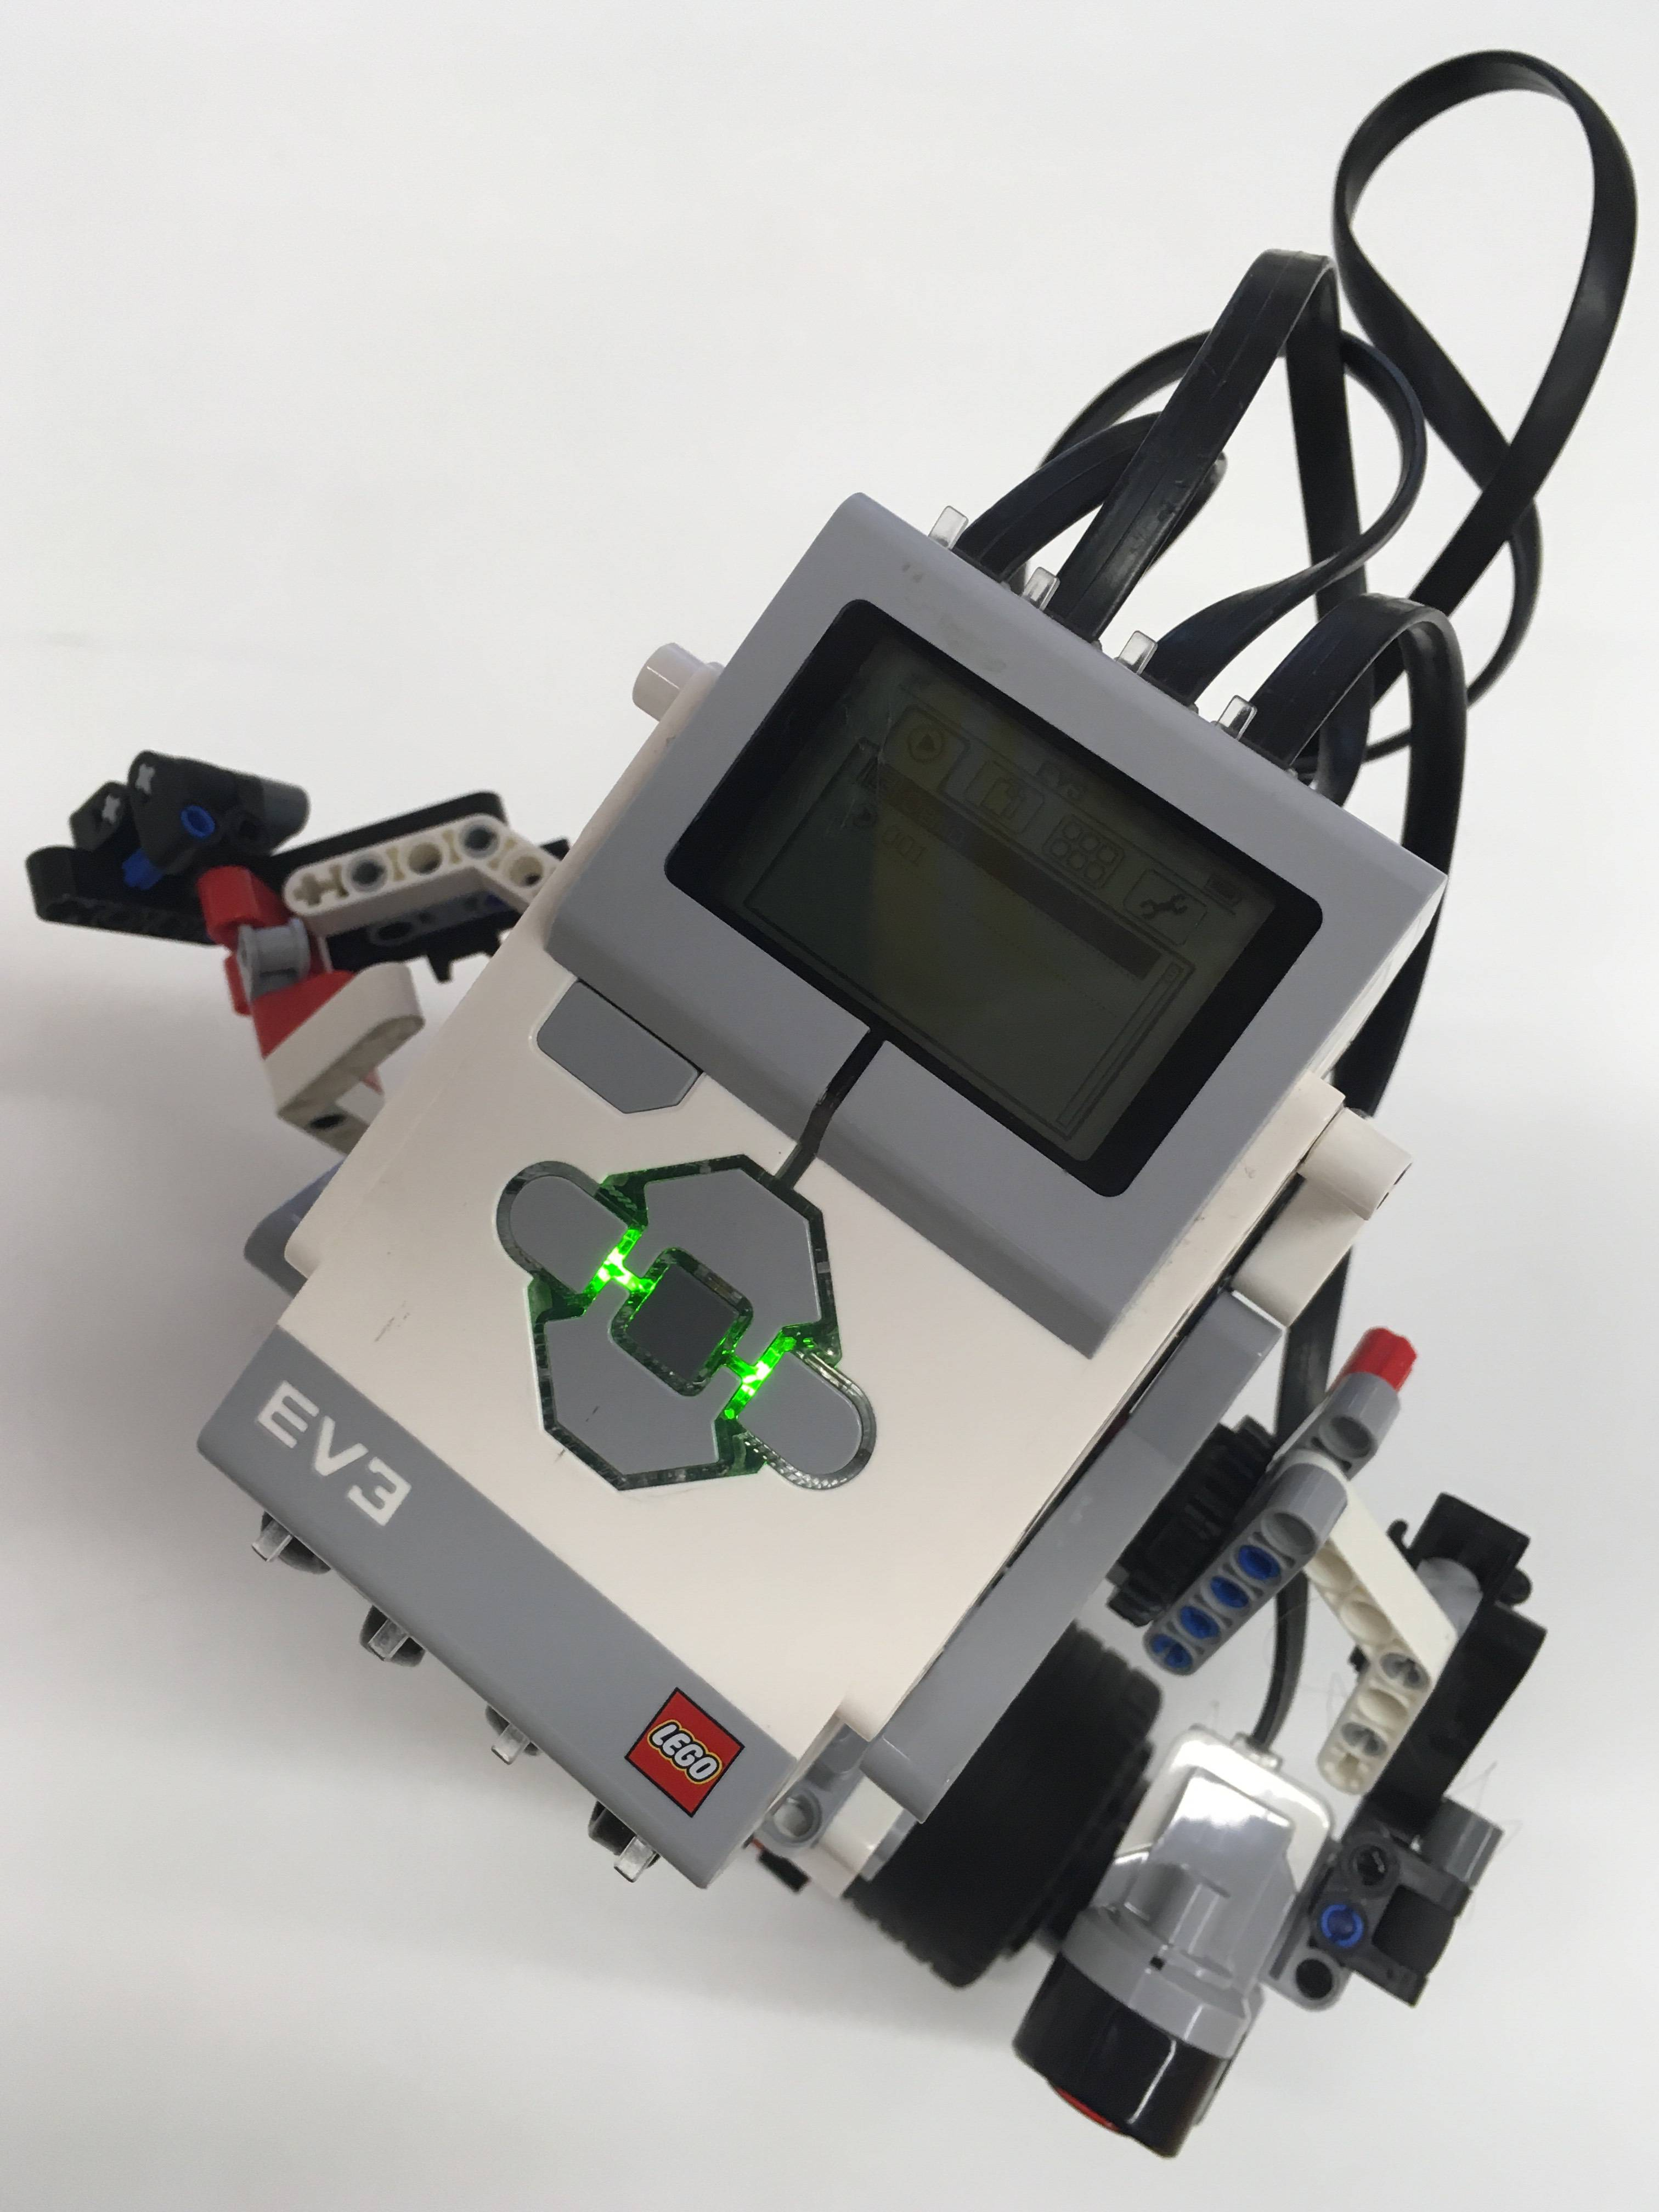
\includegraphics[width=.4\textwidth]{lego}
%}
%\hspace{\fill}
%\rightfigure{
%\hspace*{-8mm}\includegraphics[width=.55\textwidth]{ErgoJr.jpg}
%}
%\end{minipage}
%\leftcaption{\lego{} Mindstorms EV3 (Courtesy of Adi Shmorak, Intelitek)}\label{fig.lego}
%\rightcaption{Poppy Ergo Jr robotic arms (Courtesy of the Poppy Project)}\label{fig.poppy}
%\end{figure}

\smallskip

\noindent\textbf{Braços Robóticos}

Para agir em seu ambiente, o robô precisa de um \emph{atuator} que é um componente de um robô que afeta o ambiente. Muitos robôs, em particular os braços robóticos usados na indústria, afetam o ambiente por meio de ferramentas conectadas a sua extremidade móvel, ou \emph{efetores finais}, geralmente garras ou ferramentas similares (Figs.~\ref{fig.assemblyline}, \ref{fig.sortballs}, \ref{fig.robots-pulling}). Os atuadores dos robôs móveis são os motores que provocam o movimento do robô, assim como componentes como a bomba de vácuo de um aspirador.

Robôs educacionais são geralmente robôs móveis cujos únicos atuadores são seus motores e dispositivos de exibição, tais como luzes, sons ou uma tela. Os efetores finais podem ser construídos com kits robóticos ou usando componentes adicionais com robôs pré-montados, embora existam braços robóticos educacionais (Fig.~\ref{fig.poppy}). A manipulação de objetos introduz complexidade no projeto; entretanto, uma vez que os algoritmos para os efetores finais são similares aos algoritmos para robôs móveis simples, a maioria das atividades deste livro assumirá que seu robô possui apenas motores e dispositivos de exibição.

\smallskip

\noindent\textbf{Ambientes de Desenvolvimento de Software}

Todo sistema de robótica educacional inclui um \emph{ambiente de desenvolvimento de software}. A linguagem de programação pode ser uma versão de uma linguagem de programação padrão como Java ou Python. A programação é simplificada se for utilizada uma linguagem baseada em blocos, geralmente uma linguagem como Scratch ou Blockly (Fig.~\ref{fig.ide-blocks}).

\begin{figure}
\begin{center}
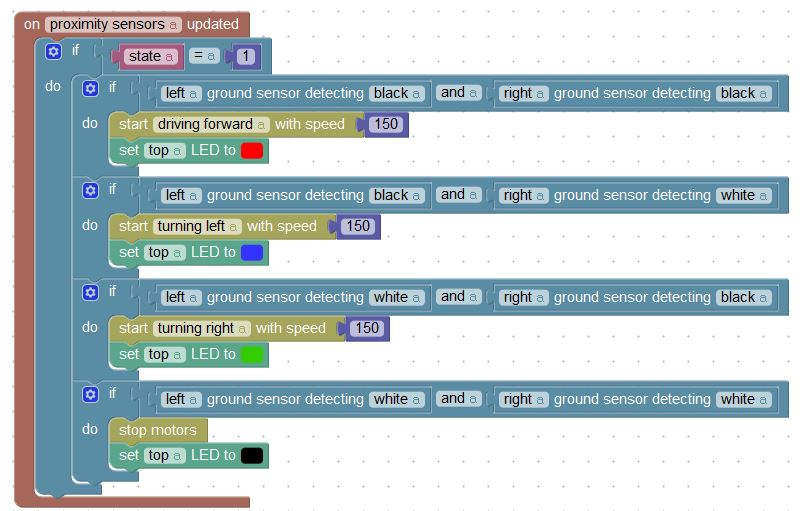
\includegraphics[width=.7\textwidth]{blockly}
\end{center}
\caption{Código em Blockly para o robô Thymio}\label{fig.ide-blocks}
\end{figure}

Para simplificar ainda mais a programação de um robô por jovens estudantes, uma notação de programação totalmente gráfica pode ser utilizada. As figuras~\ref{fig.ide-thymio} mostram VPL (Visual Programming Language), um ambiente de software gráfico para o robô Thymio. Ele utiliza pares de ação de eventos: quando o evento representado pelo bloco à esquerda ocorre, as ações nos blocos seguintes são executadas.

\begin{figure}
\begin{center}
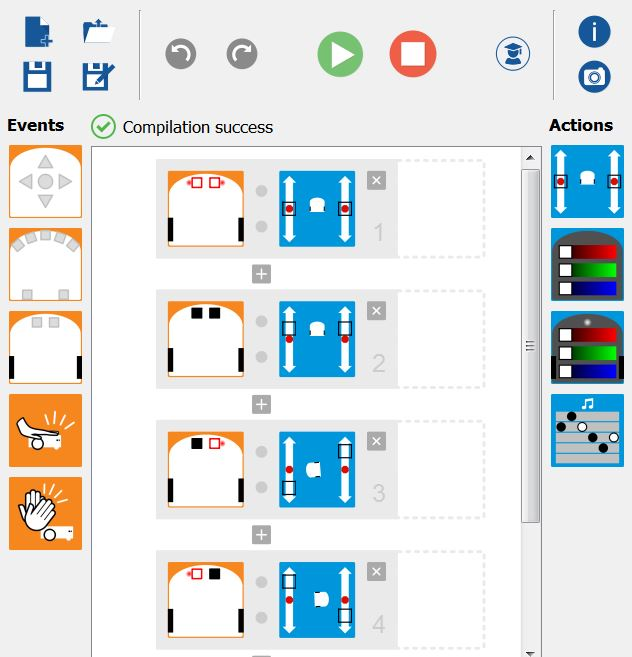
\includegraphics[width=.7\textwidth]{vpl}
\end{center}
\caption{Software VPL para o robô Thymio}\label{fig.ide-thymio}
\end{figure}

A figura~\ref{fig.ide-dash} mostra o ambiente gráfico de software para o robô Dash. Ele também utiliza eventos e ações, onde as ações são representadas por nós e os eventos são representados por setas entre os nós.

\begin{figure}
\begin{center}
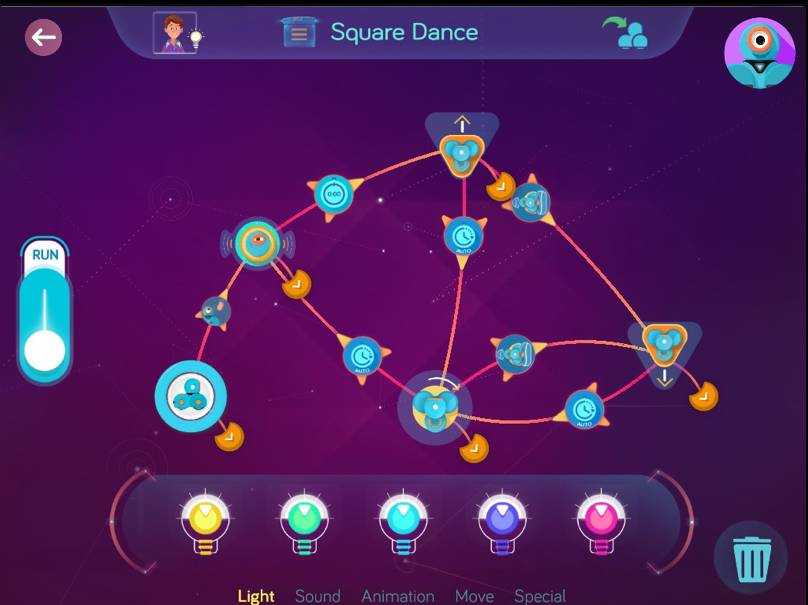
\includegraphics[width=.8\textwidth]{wonder}
\end{center}
\caption{Software Wonder para o robô Dash (Cortesia: Dash Wonder Workshop)}\label{fig.ide-dash}
\end{figure}

\section{O Robô Genérico}\label{s.generic}

Esta seção apresenta a descrição de um robô genérico que usamos para apresentar os algoritmos de robótica. As capacidades do robô genérico são semelhantes àquelas encontradas nos robôs educacionais, mas aquele que você usa pode não ter todas as capacidades assumidas nas apresentações, então você terá de improvisar. Você pode não entender todos os termos na descrição a seguir, mas é importante que a especificação seja formalizada. Mais detalhes serão fornecidos em capítulos posteriores.

\subsection{Acionamento Diferencial}

O robô é um pequeno veículo autônomo com tração diferencial, ou seja, tem duas rodas que são acionadas por motores independentes (Fig.~\ref{fig.differential}). Para fazer o robô mover-se, ajuste a potência do motor para um valor de $-100$ (potência total para trás) a $0$ (parado) até $100$ (potência total para frente). Não há relação pré-definida entre a potência do motor e a velocidade do robô. O motor pode ser conectado às rodas através de diferentes relações de transmissão, o tipo de pneus nas rodas afeta sua tração, e terreno arenoso ou lamacento pode causar o deslizamento das rodas.

\begin{figure}
\begin{center}
\begin{tikzpicture}[scale=1.2]
\pic[scale=1.5] at (0,0) { robot };
\draw[densely dotted,thick] (12mm,0) circle[radius=6pt];
\draw[->] (16mm,10mm) node[right] {\p{support (on the bottom of the robot)}} -- (13mm,3mm);
\draw[->,thick] (20mm,0) -- node[below] {\p{forward} } +(18mm,0);
\draw[raxis] (0,0) -- (0,15mm);
\draw[raxis] (0,0) -- (0,-15mm);
\draw[raxis] (0,0) -- (11pt,0);
\draw[raxis] (0,0) -- (-11pt,0);
\end{tikzpicture}
\end{center}
\caption{Robô com acionamento diferencial\label{fig.differential}}
\end{figure}

A figura~\ref{fig.differential} mostra uma visão do robô de cima. A frente do robô é a curva para a direita, que é também a direção do movimento do robô para frente. As rodas (retângulos pretos) estão do lado esquerdo e direito da parte traseira do corpo do robô. O círculo negro representa o ponto sobre o eixo a meio caminho entre as rodas. Quando o robô gira, ele gira em torno de um eixo vertical sobre este ponto. Para estabilidade, em direção à frente do robô há um suporte ou roda não atuada.

\begin{quote}
\begin{center}
\textbf{Desenho Mecânico}
\end{center}
Uma linha tracejada é a notação padrão na engenharia mecânica para o eixo de simetria em um componente, como uma roda. Quando a visão lateral de uma roda é exibida, a intersecção dos dois eixos de simetria denota o eixo de rotação que é perpendicular ao plano da página. Para evitar a desordem dos diagramas, simplificamos a notação mostrando apenas linhas quebradas para um \emph{eixo de rotação} de um componente, como uma roda. Além disso, a intersecção denotando um eixo perpendicular é normalmente abreviada para uma cruz, possivelmente contida dentro da roda ou de seu eixo.
\end{quote}

O acionamento diferencial tem várias vantagens: é simples, pois possui apenas dois motores sem componentes adicionais para a direção e permite que o robô gire no lugar. Em um carro, duas rodas são acionadas juntas (ou quatro rodas são acionadas em pares) e há um mecanismo complexo separado para direção chamado \emph{direção Ackermann}. Como um carro não pode virar no lugar, os motoristas devem realizar manobras complicadas como estacionamento paralelo; motoristas humanos aprendem prontamente a fazer isso, mas tais manobras são difíceis para um sistema autônomo. Um robô autônomo precisa realizar manobras intrincadas com movimentos muito simples, e é por isso que a tração diferencial é a configuração preferida: ele pode facilmente virar para qualquer direção e depois se mover nessa direção.

A principal desvantagem de um sistema de acionamento diferencial é que ele requer um terceiro ponto de contato com o solo, ao contrário de um carro que já tem quatro rodas para apoiá-lo e, portanto, pode mover-se facilmente em terrenos difíceis. Outra desvantagem é que ele não pode deslocar-se lateralmente sem girar. Existem configurações que permitem que um robô se mova lateralmente (Sect.~\ref{s.holonomic}), mas elas são complexas e caras. O acionamento diferencial também é usado em veículos sobre esteiras, como equipamentos de terraplenagem e tanques militares. Estes veículos podem manobrar em terrenos extremamente acidentados, mas as esteiras produzem muito atrito, de modo que o movimento é lento e não preciso.

\begin{quote}
\begin{center}
\textbf{Ajuste de Potência ou Ajuste de Velocidade}
\end{center}
A potência fornecida por um motor é regulada por um \emph{"acelerador"}, tal como um pedal em um carro ou alavancas em um avião ou barco. Os motores elétricos usados em robôs móveis são controlados pela amplitude da tensão aplicada aos motores usando uma técnica chamada PWM, sigla em inglês para \emph{Modulação por Largura de Pulso}. Em muitos robôs educacionais, algoritmos de controle como os descritos no Cap.~\ref{ch.control}, são usados para garantir que os motores girem a uma velocidade {desejada especificada}. Como estamos interessados em conceitos e algoritmos para projetar robôs, iremos expressar algoritmos em termos de fornecimento de potência e lidar separadamente com o controle de velocidade.
\end{quote}

\subsection{Sensores de Proximidade}

O robô possui sensores de proximidade horizontais que podem detectar um objeto próximo a ele. Existem muitas tecnologias que podem ser usadas para construir estes sensores, tais como infravermelho, laser, ultra-som; o robô genérico representa robôs que usam qualquer uma destas tecnologias. Nós especificamos que os sensores têm as seguintes capacidades: Um sensor de proximidade horizontal pode medir a distância (em centímetros) entre o robô e um objeto e o ângulo (em graus) entre a frente do robô e o objeto. A figura~\ref{fig.generic-sensor} mostra um objeto localizado a $3\,$ cm do centro do robô em um ângulo de $45^{\circ}$ da direção em que o robô está apontando.\footnote{Ver Apêndice~\ref{ch.units} sobre as convenções para medição de ângulos.}

\begin{figure}
\begin{minipage}{.45\textwidth}
\begin{tikzpicture}
\pic[scale=1.2] at (0,0) { robot };
\draw[->] (0,0) -- node[sloped,above] {$3\,$cm} (45:2.5cm) node[above right=-4pt] {$\bullet$};
\draw[dashed] (0,0) node[above,xshift=20pt] {$45^{\circ}$}-- (2.5,0);
\draw (10pt,0) arc [start angle=0, end angle=45, radius=10pt];
\fill[gray] (0,0) circle[radius=4pt];
\end{tikzpicture}
\caption{Robô com um sensor rotativo (ponto cinza)}
\label{fig.generic-sensor}
\end{minipage}
\hspace{\fill}
\begin{minipage}{.45\textwidth}
\begin{tikzpicture}
\pic[scale=1.2] at (0,0) { robot2 };
\end{tikzpicture}
\caption{Robô com dois sensores de solo na parte inferior do robô (retângulos cinza)}
\label{fig.generic-ground}
\end{minipage}
\end{figure}

%\begin{figure}
%\subfigures
%\leftfigure{
%\begin{tikzpicture}
%\pic[scale=1.2] at (0,0) { robot };
%\draw[->] (0,0) -- node[sloped,above] {$3\,$cm} (45:2.5cm) node[above right=-4pt] {$\bullet$};
%\draw[dashed] (0,0) node[above,xshift=20pt] {$45^{\circ}$}-- (2.5,0);
%\draw (10pt,0) arc [start angle=0, end angle=45, radius=10pt];
%\fill[gray] (0,0) circle[radius=4pt];
%\end{tikzpicture}
%}
%\hspace{\fill}
%\rightfigure{
%\begin{tikzpicture}
%\pic[scale=1.2] at (0,0) { robot2 };
%\end{tikzpicture}
%}
%\leftcaption{Robot with a rotating sensor (gray dot)\label{fig.generic-sensor}}
%\rightcaption{Robot with two ground sensors on the bottom of the robot (gray rectangles)}\label{fig.generic-ground}
%\end{figure}

Na prática, um robô educacional terá um pequeno número de sensores, portanto pode não será capaz de detectar objetos em todas as direções. Além disso, os sensores baratos não serão capazes de detectar objetos que estão longe e suas medidas não serão precisas. As medições também serão afetadas por fatores ambientais como o tipo de objeto, a luz ambiente, e assim por diante. Para simplificar nossos algoritmos, não assumimos nenhuma limitação pré-definida, mas ao implementar os algoritmos, você terá que levar em conta tais limitações.

\subsection{Sensores de Solo}

\emph{Os sensores de solo} são montados na parte inferior do robô. Como estes sensores estão muito próximos ao solo, não há significado de distância ou ângulo; em vez disso, o sensor mede o brilho da luz refletida do solo em valores arbitrários entre $0$ (totalmente escuro) e $100$ (totalmente claro). O robô genérico tem dois sensores de solo montados em sua parte frontal inferior (Fig.~\ref{fig.generic-ground}), embora às vezes apresentemos algoritmos que utilizam apenas um sensor. A figura mostra uma vista superior do robô, embora os sensores de solo estejam na parte inferior do mesmo.

\subsection{Computador Embarcado}\label{s.embedded}

O robô é equipado com um \emph{computador embarcado} (Fig.~\ref{fig.computer}). A especificação precisa do computador não é importante, mas nós assumimos certas capacidades. O computador pode ler os valores dos sensores e definir a potência dos motores. Há uma maneira de exibir informações em uma pequena tela ou usando luzes coloridas. Os sinais e dados podem ser inseridos no computador usando botões, um teclado ou um controle remoto.

\begin{figure}
\begin{center}
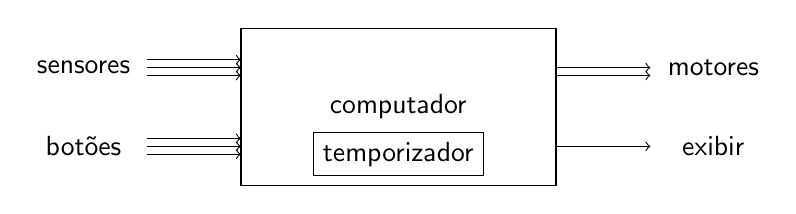
\begin{tikzpicture}
\node[draw,rectangle,minimum width=4cm,minimum height=2cm] at (0,0) {\textsf{computador}};
\node[draw,rectangle] at (0,-.6) {\textsf{temporizador}};
\node at (-4,.5) {\textsf{sensores}};
\node at (-4,-.5) {\textsf{botões}};
\draw[->] (-3.2,.4) -- (-2,.4);
\draw[->] (-3.2,.5) -- (-2,.5);
\draw[->] (-3.2,.6) -- (-2,.6);
\draw[->] (-3.2,-.4) -- (-2,-.4);
\draw[->] (-3.2,-.5) -- (-2,-.5);
\draw[->] (-3.2,-.6) -- (-2,-.6);
\node at (4,.5) {\textsf{motores}};
\node at (4,-.5) {\textsf{exibir}};
\draw[->] (2,.4) -- (3.2,.4);
\draw[->] (2,.5) -- (3.2,.5);
\draw[->] (2,-.5) -- (3.2,-.5);
\end{tikzpicture}
\caption{Computador embarcado}\label{fig.computer}
\end{center}
\end{figure}

Os dados são introduzidos no computador por \emph{eventos} como, por exemplo, o toque de um botão. A ocorrência de um evento provoca a execução de um procedimento chamado de \emph{gerenciador de eventos}. O evento pode ser detectado pelo hardware, em cujo caso o termo \emph{interrupção} é usado, ou pode ser detectado pelo software, geralmente, por amostragem (em inglês, \emph{polling}), onde o sistema operacional verifica a existência de eventos em intervalos pré-definidos. Quando a tarefa do gerenciador de eventos é encerrada, a execução do programa principal é retomada.

Os gerenciadores de eventos são diferentes dos programas sequenciais que têm uma instrução inicial que insere dados e uma instrução final que exibe a saída, porque os gerenciadores de eventos são executados em resposta a eventos imprevisíveis. O tratamento de interrupções através do gerenciador de eventos é usado para implementar interfaces gráficas de usuário em computadores e smartphones: ao clicar ou tocar em um ícone, um gerenciador de eventos é executado. Em um robô, um evento pode ser uma entrada discreta como tocar uma tecla. Eventos também podem ocorrer quando um valor contínuo como o valor lido por um sensor ultrapassa um limite pré-definido, em inglês chamado de \emph{threshold}.

O computador inclui um \emph{temporizador} que funciona como um cronômetro em um smartphone. Um temporizador é uma variável que é \emph{ajustada} para um período de tempo, por exemplo, $0,5$ segundo, que é representado como um número inteiro de milissegundos ou microssegundos ($0,5$ segundo é igual a $500$ milissegundos). O relógio de hardware do computador causa uma interrupção em intervalos fixos e o sistema operacional decrementa o valor do temporizador. Quando seu valor chega a zero, dizemos que o temporizador \emph{expirou}; ocorre uma interrupção.

Os temporizadores são usados para implementar eventos que se repetem, como piscar uma luz. Eles também são usados para realizar a amostragem de sinais (\emph{polling}), uma alternativa aos gerenciadores de eventos: em vez de realizar um cálculo quando um evento ocorre, os sensores são lidos periodicamente. Mais precisamente, a amostragem ocorre como um gerenciador de eventos quando um timer expira, mas o projeto de software usando amostragem pode ser bem diferente do projeto de software baseado em eventos.

\section{O Formalismo Algorítmico}\label{s.alg-formalism}

Algoritmos que são implementados como programas de computador são usados pelo computador embarcado para controlar o comportamento do robô. Não fornecemos programas em nenhuma linguagem de programação específica; em vez disso, os algoritmos são apresentados em \emph{pseudo-código}\footnote{N. do T.: Preferimos não traduzir os nomes de variáveis nem os comandos usados nos pseudo-códigos para o português já que os termos em inglês guardam semelhança com os comandos de linguagens de programação de alto nível e os códigos-exemplo disponíveis.}, um formato estruturado usando uma combinação de linguagem natural, matemática e estruturas de programação. O algoritmo~\ref{alg.integer-mult} é um algoritmo simples para multiplicação de números inteiros usando adição repetida. A entrada do algoritmo é um par de números inteiros e a saída é o produto dos dois valores de entrada. O algoritmo declara três variáveis inteiras \p{x}, \p{a}, \p{b}. Há cinco declarações na parte executável. Um recuo (ou indentação) é usado para indicar o escopo do laço (como na linguagem de programação Python). Uma seta é usada para indicar atribuição, para que os símbolos familiares $=$ e $\neq$ possam ser usados para igualdade e desigualdade nas fórmulas matemáticas.\footnote{Muitas linguagens de programação usam \texttt{=} para atribuição, \texttt{==} para testar igualdade e \texttt{!=} para testar desigualdade. Isto é confuso porque a igualdade $x=y$ é simétrica, mas a atribuição não é \texttt{x=x+1}. Preferimos manter a notação matemática.}

\begin{figure}
\begin{alg}{Multiplicação inteira}{integer-mult}           
&\idv{}integer x \ass 0&\\
&\idv{}integer a, b&\\
\hline
\stl{}&a \ass entrada de um inteiro&\\
\stl{}&b \ass entrada de um inteiro não negativo&\\
\stl{}&while b $\neq$ 0&\\
\stl{}&\idc{} x \ass x $+$ a&// Soma o valor de a com x\\
\stl{}&\idc{} b \ass b $-$ 1&// \ \ para cada b\\
\end{alg}
\end{figure}

A potência do motor é definida usando declarações de atribuição:
\begin{quote}
\p{left-motor-power} \ass $50$\\
\p{right-motor-power} \ass $-50$
\end{quote}

Definimos nossos sensores de proximidade como retornando a distância a um objeto detectado e seu ângulo em relação à direção dianteira do robô, mas muitas vezes será mais conveniente usar expressões de linguagem natural como, por exemplo
\begin{quote}
\p{when object detected in front (quando objeto detectado em frente)}\\
\p{when object not detected in back (quando objeto não detectado a trás)}
\end{quote}

\section{Uma Visão Geral do Conteúdo do Livro}\label{s.overview}

Os primeiros seis capítulos formam o núcleo dos conceitos e algoritmos de robótica.
\begin{description}
\item [\textbf{Capítulo \ref{ch.basic} Robôs e Suas Aplicações}] Este capítulo examina e classifica os robôs. Também especifica os robôs genéricos e os formalismos usados para apresentar algoritmos neste livro.

\item [\textbf{Capítulo \ref{ch.sensors} Sensores}] Os robôs são mais do que aparelhos controlados remotamente, como um aparelho de televisão. Eles mostram um comportamento autônomo baseado na detecção de objetos em seu ambiente usando sensores. Este capítulo dá uma visão geral dos sensores usados pelos robôs e explica os conceitos de alcance, resolução, precisão e exatidão. Também discute a não-linearidade dos sensores e como lidar com ela.

\item [\textbf{Capítulo \ref{ch.reactive} Comportamento Reativo}] Quando um robô autônomo detecta um objeto em seu ambiente, ele reage alterando seu comportamento. Este capítulo introduz algoritmos que fazem com que um robô mude diretamente seu comportamento com base na entrada de seus sensores. Os veículos Braitenberg são exemplos simples, porém elegantes, de comportamento reativo. O capítulo apresenta diversas variantes de algoritmos seguidores de linha.

\item [\textbf{Capítulo \ref{ch.fmg} Máquinas de Estado Finitas}] Um robô pode estar em diferentes estados, sendo que sua reação à entrada de seus sensores depende não só destes valores, mas também do estado atual. Máquinas de estado finitas são um formalismo para descrever estados e as transições entre eles que dependem da ocorrência de eventos.

\item [\textbf{Capítulo \ref{ch.motion} Movimentação de Robôs e Odometria}] Robôs autônomos exploram seu ambiente executando ações. Dificilmente passa um dia sem um relatório sobre a experiência com veículos autônomos. Este capítulo revisa conceitos relacionados ao movimento (distância, tempo, velocidade, aceleração), e depois apresenta a odometria, o método fundamental que um robô utiliza para se mover de uma posição para outra. A odometria está sujeita a erros significativos e é importante entender sua natureza.

A segunda parte do capítulo dá uma visão geral dos conceitos avançados de movimentação de robôs: codificadores (em inglês, \emph{encoders}) de roda e sistemas de navegação inercial que podem melhorar a precisão da odometria, e graus de liberdade e holonomia que afetam o planejamento do deslocamento de robôs.

\item [\textbf{Capítulo \ref{ch.control} Controle}] Um robô autônomo é um sistema de controle de circuito fechado porque a entrada de dados de seus sensores afeta seu comportamento que, por sua vez, afeta o que é medido pelos sensores. Por exemplo, um carro que se aproxima de um semáforo pode frear mais forte à medida que se aproxima do semáforo. Este capítulo descreve a matemática dos sistemas de controle que garantem um comportamento ideal: o carro realmente pára no semáforo e a frenagem é gradual e suave.
\end{description}

Um robô móvel autônomo deve de alguma forma navegar de uma posição inicial a uma posição desejada, por exemplo, para levar medicamentos da farmácia de um hospital ao paciente. A navegação é um problema fundamental na robótica que é difícil de resolver. Os quatro capítulos seguintes apresentam algoritmos de navegação em vários contextos.
\begin{description}
\item [\textbf{Capítulo \ref{ch.obstacle} Navegação Local: Evasão de Obstáculos}] O requisito mais básico de um robô móvel é que ele não bata em paredes, pessoas e outros obstáculos. Isto é chamado de navegação \emph{local} porque trata da vizinhança imediata do robô e não de objetivos que o robô está tentando alcançar. O capítulo começa com algoritmos de seguimento de parede, que permitem que um robô se mova em torno de um obstáculo; tais algoritmos são similares aos algoritmos para navegar em um labirinto. O capítulo descreve um algoritmo probabilístico que simula a navegação por uma colônia de formigas em busca de uma fonte de alimento.
\item [\textbf{Capítulo \ref{ch.local} Localização}] Antes de cada smartphone incluir a navegação por GPS, nós costumávamos navegar com mapas impressos em papel. Um problema difícil é a localização: você pode determinar sua posição atual no mapa? Os robôs móveis devem resolver o mesmo problema de localização, muitas vezes sem o benefício da visão. O capítulo descreve a localização através de cálculos trigonométricos a partir de posições conhecidas. A isto se seguem seções sobre a localização probabilística: um robô pode detectar um ponto de referência, mas pode haver muitos pontos de referência similares no mapa. Ao atribuir probabilidades e atualizá-las à medida em que se move através do ambiente, o robô pode eventualmente determinar sua posição com relativa certeza.

\item [\textbf{Capítulo \ref{ch.mapping} Mapeamento}] Mas de onde vem o mapa? Mapas de ruas precisos estão prontamente disponíveis, mas um aspirador robótico não tem um mapa de seu apartamento. Um robô subaquático é usado para explorar um ambiente desconhecido. Para realizar a localização o robô precisa de um mapa, mas para criar um mapa de um ambiente desconhecido o robô precisa se localizar, no sentido de que tem que saber até onde se deslocou de um ponto do ambiente para outro. A solução é realizar a localização e o mapeamento simultâneos. A primeira parte do capítulo descreve um algoritmo para explorar um ambiente para determinar a localização de obstáculos. Em seguida, é apresentado um algoritmo simplificado para localização e mapeamento simultâneos.

\item [\textbf{Capítulo \ref{ch.map-based} Navegação com base em Mapeamento}] Agora que o robô tem um mapa, suponha que lhe seja atribuída uma tarefa que requeira que ele passe de uma posição inicial para uma posição desejada. Que rota ele deve tomar? Este capítulo apresenta dois algoritmos para o planejamento do caminho: O algoritmo de Dijkstra, um algoritmo clássico para encontrar o caminho mais curto em um grafo, e o algoritmo \astar{}, uma versão mais eficiente do algoritmo de Dijkstra que usa informações heurísticas.
\end{description}

Os capítulos seguintes apresentam tópicos avançados em robótica. Eles são independentes uns dos outros para que você possa selecionar quais deles estudar e em que ordem.
\begin{description}
\item [\textbf{Chapter \ref{ch.fuzzy} Controle de Lógica Fuzzy}] Os algoritmos de controle clássico (Cap.~\ref{ch.control}) exigem a especificação de um valor desejado preciso: um sistema de aquecimento precisa da temperatura desejada de uma sala e um sistema de \emph{cruise control} precisa da velocidade desejada de um carro. Uma abordagem alternativa chamada lógica difusa (ou \emph{fuzzy}) usa especificações imprecisas como muito frio, frio, morno, quente, ou muito lento, lento, rápido, muito rápido. Este capítulo apresenta a lógica fuzzy e mostra como ela pode ser usada para controlar um robô que se aproxima de um objeto.

\item [\textbf{Chapter \ref{ch.image} Processamento de Imagem}] A maioria dos sensores usados em robôs medem distâncias e ângulos usando lasers, som ou luz infravermelha. Nós, humanos, confiamos principalmente em nossa visão. Câmeras digitais de alta qualidade são baratas e encontradas em todos os smartphones. A dificuldade é processar e interpretar as imagens captadas pela câmera, algo que nosso cérebro faz instantaneamente. O processamento digital de imagens tem sido objeto de extensa pesquisa e seus algoritmos são usados em robôs avançados que podem proporcionar o poder computacional necessário. Neste capítulo pesquisamos os algoritmos de processamento de imagem e mostramos como um robô educacional pode demonstrar os algoritmos mesmo sem uma câmera.

\item [\textbf{Chapter \ref{ch.neural} Redes Neurais}] Os robôs autônomos em ambientes altamente complexos não podem ter algoritmos para todas as situações possíveis. Um veículo autônomo não pode conhecer antecipadamente todos os diferentes veículos e configurações de veículos que ele encontra na estrada. Os robôs autônomos devem aprender com sua experiência e este é um tópico fundamental na inteligência artificial que vem sendo estudado há muitos anos. Este capítulo apresenta uma abordagem do aprendizado: redes neurais artificiais modeladas com base nos neurônios de nossos cérebros. Uma rede neural usa algoritmos de aprendizagem para modificar seus parâmetros internos de modo a se adaptar continuamente a novas situações que encontra.

\item [\textbf{Chapter \ref{ch.machine} Aprendizagem de Máquina}] Outra abordagem da aprendizagem é uma técnica estatística chamada aprendizagem de máquina. Este capítulo descreve dois algoritmos para distinguir entre duas alternativas; por exemplo, distinguir entre um semáforo que é vermelho e um que é verde. O primeiro algoritmo, chamado análise linear discriminante, é baseado nos meios e variações de um conjunto de amostras. O segundo algoritmo usa perceptrons, uma forma de rede neural que pode distinguir entre alternativas mesmo quando as amostras não satisfazem as suposições estatísticas necessárias para a análise linear discriminante.

\item [\textbf{Chapter \ref{ch.swarm} Robótica de Enxame}] Se você precisa melhorar o desempenho de um sistema, muitas vezes é mais fácil usar múltiplas instâncias de um componente em vez de tentar melhorar o desempenho de um componente individual. Considere um problema como o monitoramento de uma área para medir os níveis de poluição. Você pode usar um único robô muito rápido (e caro), mas pode ser mais fácil usar vários robôs, cada um dos quais mede a poluição em uma área pequena. Isto é chamado de robótica de enxame por analogia com um enxame de insetos que pode encontrar o melhor caminho entre seu ninho e uma fonte de alimento. O problema fundamental na robótica de enxame, como em todos os sistemas concorrentes, é desenvolver métodos de coordenação e comunicação entre os robôs. Este capítulo apresenta duas dessas técnicas: troca de informações e interações físicas.

\item [\textbf{Chapter \ref{ch.kinematics} Cinemática de Manipuladores Robóticos}] Robôs educacionais são pequenos robôs móveis que se movem em uma superfície bidimensional. Há robôs móveis que se movem em três dimensões: aeronaves robóticas e submarinos. A matemática e os algoritmos para o movimento tridimensional foram desenvolvidos em outro campo central da robótica: os manipuladores, que são usados extensivamente na fabricação. Este capítulo apresenta um tratamento simplificado dos conceitos fundamentais dos manipuladores robóticos (cinemática direta e inversa, rotações, transformações homogêneas) em duas dimensões, bem como uma amostra de rotações tridimensionais.
\end{description}

Há dois apêndices:
\begin{description}
\item [\textbf{Anexo \ref{ch.units} Unidades de Medida}] Este apêndice contém a Tabela A.1 com unidades de medidas. A Tabela A.2 fornece prefixos que são usados com essas unidades.

\item [\textbf{Anexo \ref{ch.math} Derivações Matemáticas e Tutoriais}]. Este capítulo contém tutoriais que revisam alguns dos conceitos matemáticos utilizados no livro. Além disso, algumas das derivações matemáticas detalhadas foram coletadas aqui para não quebrar o fluxo do texto.
\end{description}

\section{Sumário}

Os robôs são encontrados em toda parte: em fábricas, residências e hospitais, e até mesmo no espaço. Muita pesquisa e desenvolvimento está sendo investida no desenvolvimento de robôs que interagem diretamente com os seres humanos. Robôs são usados nas escolas a fim de aumentar a motivação dos estudantes para estudar STEM e como ferramenta pedagógica para ensinar STEM em um ambiente concreto. O foco deste livro é o uso de robôs educacionais para aprender algoritmos robóticos e para explorar seu comportamento.

A maioria dos robôs educacionais tem um projeto semelhante: um pequeno robô móvel que utiliza acionamento diferencial e sensores de proximidade. Para tornar este livro independente de plataforma, definimos um robô genérico com estas propriedades. Os algoritmos apresentados neste livro para o robô genérico devem ser fáceis de implementar em robôs educacionais, embora robôs diferentes tenham capacidades diferentes em termos de desempenho de seus motores e sensores. Os algoritmos são apresentados em pseudo-código independente de linguagem de programação, que deve ser fácil de traduzir para qualquer linguagem textual ou gráfica que seu robô suporte.

\section{Leitura Adicional}

Para uma visão geral não técnica da robótica com ênfase na robótica de inspiração biológica e humanóide, veja Winfield~\cite{vsi}.

A Organização Internacional para Padronização (ISO)\footnote{ISO é seu nome oficial abreviado, e não uma sigla em nenhuma de suas três línguas oficiais: inglês, francês e russo.} publica normas para robótica. Em seu website \url{https://www.iso.org/} você pode encontrar o catálogo de robótica (ISO/TC 299) e definições formais de conceitos de robótica: ISO 8373:2012 Robôs e Dispositivos Robóticos---Vocabulário e ISO 19649:2017 Robôs Móveis---Vocabulário.

Os tópicos deste livro são apresentados com mais detalhes em livros didáticos avançados sobre robótica, tais como \cite{dudek,siegwart}. Seus capítulos introdutórios dão muitos exemplos de robôs.

Os robôs educacionais vêm com documentação de suas capacidades e ambientes de desenvolvimento de software. Há também livros didáticos baseados em robôs específicos, por exemplo, \cite{trobaugh} a programação dos kits de robótica \lego{} Mindstorms e \cite{kumar} sobre o uso do Python para programar os robôs Scribbler. O projeto da linguagem de programação visual (VPL) é apresentado em \cite{shin2014idc}.

Pseudocódigo é frequentemente usado em livros didáticos sobre estruturas de dados e algoritmos, a partir do clássico livro didático \cite{aho}. O estilo usado aqui é baseado em \cite{pcdp2}.

